\documentclass[12pt,titlepage,a4paper]{report}
\usepackage[margin=1.25in]{geometry}
\usepackage{graphicx,amsmath,blindtext,minted}

%% Variables definition
\newcommand{\vSubject}{Advanced Database Course}
\newcommand{\vSubtitle}{Library Management System Report}
\newcommand{\vName}{Muhammad Baihaqi Aulia Asy'ari}
\newcommand{\vNIM}{2241720145}
\newcommand{\vClass}{2I}
\newcommand{\vGroup}{Batam}
\newcommand{\vDepartment}{Information Technology}
\newcommand{\vStudyProgram}{D4 Informatics Engineering}

%% [START] Tikz related stuff
\usepackage{tikz}
\usetikzlibrary{svg.path,calc,shapes.geometric,shapes.misc}
\tikzstyle{terminator} = [rectangle, draw, text centered, rounded corners = 1em, minimum height=2em]
\tikzstyle{preparation} = [chamfered rectangle, chamfered rectangle sep=0.75em, draw, text centered, minimum height = 2em]
\tikzstyle{process} = [rectangle, draw, text centered, minimum height=2em]
\tikzstyle{decision} = [diamond, aspect=2, draw, text centered, minimum height=2em]
\tikzstyle{data}=[trapezium, draw, text centered, trapezium left angle=60, trapezium right angle=120, minimum height=2em]
\tikzstyle{connector} = [line width=0.25mm,->]
%% [END] Tikz related stuff

%% [START] Fancy header related stuff
\usepackage{fancyhdr}
\pagestyle{fancy}
\setlength{\headheight}{15pt} % compensate fancyhdr style
\fancyhead{}
\fancyfoot{}
\fancyfoot[L]{\thepage}
\fancyfoot[R]{\textit{\vSubject - \vSubtitle}}
\renewcommand{\footrulewidth}{0.4pt}% default is 0pt, overline for footer

\fancypagestyle{plain}{
    \fancyhf{}
    \setlength{\headheight}{15pt} % compensate fancyhdr style
    \fancyhead{}
    \fancyfoot{}
    \fancyfoot[L]{\thepage}
    \fancyfoot[R]{\textit{\vSubject - \vSubtitle}}
    \renewcommand{\footrulewidth}{0.4pt}% default is 0pt, overline for footer
}
%% [END] Fancy header related stuff

%% [START] Custom tabular command related stuff
\usepackage{tabularx}
\newcommand{\details}[2]{
    #1 & #2  \\
}
%% [END] Custom tabular command related stuff

%% [START] Figure related stuff
\newcommand{\image}[3][1]{
    \begin{figure}[h]
        \centering
        \includegraphics[#1]{#2}
        \caption{#3}
        \label{#3}
    \end{figure}
}
%% [END] Figure related stuff

%%
\usepackage{pgf-umlcd}

\renewcommand{\umldrawcolor}{black}
\renewcommand{\umlfillcolor}{white}
%%

%% [BEGIN] Custom enumerator
\usepackage{enumitem}
%% [END] Custom enumerator

%% [BEGIN] Paragraph indent
\usepackage{indentfirst}
%% [END] Paragraph indent

\renewcommand\thesection{\Roman{section}.}
\renewcommand\thesubsection{\alph{subsection}.}

\usepackage{rotating}

%% [BEGIN] URL
\usepackage{hyperref}
\hypersetup{
    colorlinks=true,
    linkcolor=blue,
    filecolor=magenta,      
    urlcolor=cyan,
    pdftitle={Overleaf Example},
    pdfpagemode=FullScreen,
    }

\urlstyle{same}
%% [END] URL

\begin{document}
\begin{titlepage}
    \centering
    \vfill
    {\bfseries\LARGE
        \vSubject\\
        \vskip0.25cm
        \vSubtitle
    }
    \vfill
    
\includegraphics[width=6cm]{images/polinema-logo.png}
    \vfill
    {
        \textbf{Group}\\
        \vGroup\\
        \vspace{0.5cm}
        \textbf{Group Members}\\
        \vspace{0.5cm}
        \begin{tabular}{l l}
            Muhammad Baihaqi Aulia Asy'ari  & \textbf{2241720145} \\
            Athriya Genferin                & \textbf{2241720075} \\
            Susila Fajar Bahiy'aqil         & \textbf{2241720245} \\            
        \end{tabular}
        \\
        \vspace{0.5cm}
        \textbf{Department}\\
        \vDepartment\\
        \vskip0.5cm
        \textbf{Study Program}\\
        \vStudyProgram
        \vskip0.5cm
        \textbf{Malang State Polytechnic}\\
        2023
    }
\end{titlepage}

\newpage

\section{Abstract}
This assignment entails the development of a comprehensive Library Management Software System, as mandated by the requirements of an advanced database course assignment. The assignment revolves around the creation of a functional system for a public library using Microsoft SQL Server. The primary objective is to empower librarians with a robust tool for efficient management of books, patrons, loans, and fines. The assignment necessitates the implementation of a database structure comprising a minimum of six tables with their respective attributes.

The core focus is on the integration of a web-based application that seamlessly interacts with the underlying SQL Server Database. The primary outcome sought is the establishment of a platform capable of performing Create, Read, Update, and Delete (CRUD) operations on the database. To achieve this, the development involves the creation of essential functions, stored procedures, and triggers, all designed to facilitate the seamless execution of CRUD operations.

This case study scenario serves as a real-world application of advanced database concepts, requiring the synthesis of database design, SQL proficiency, and web development skills. The successful completion of this assignment not only fulfills the academic requirements but also delivers a practical and functional solution for library management, showcasing the integration of theoretical knowledge into a tangible, user-friendly web application.

\newpage

\tableofcontents

\newpage

\chapter{Introduction}
\section{Background}
The inception of this assignment is rooted in the academic context of our advanced database course. Our team received a comprehensive assignment tasking us with the development of a Library Management Software System for a public library, leveraging the capabilities of Microsoft SQL Server.

The assignment aims to assess our understanding and application of advanced database concepts, requiring the implementation of a database structure encompassing at least six tables with specific attributes. Furthermore, the assignment necessitates the integration of a web-based application that proficiently interacts with the underlying SQL Server Database, enabling seamless CRUD operations.

This assignment serves as a practical exercise to synthesize theoretical knowledge into a tangible, real-world solution. The objective is not only to meet the academic requirements of the course but also to demonstrate the practical application of advanced database principles in developing a functional and user-friendly web application.

\section{Objectives and Goals of the Website}
The primary objective of the website is to establish an efficient Library Management Software System, enabling librarians to seamlessly manage books, patrons, loans, and fines. The website aims to provide a user-friendly interface with robust Create, Read, Update, and Delete (CRUD) functionality. Librarians should be able to easily add, retrieve, update, and delete information related to books, patrons, and loans through the web application.

Ensuring the integrity and security of the underlying SQL Server Database is a key goal. The website should incorporate sound database design principles to maintain data accuracy and implement security measures to safeguard sensitive information. As a critical aspect of the assignment's objectives, adherence to the assignment requirements outlined in the advanced database course is paramount. This includes the creation of at least six tables with their attributes to facilitate CRUD operations.

\chapter{Overview}

\section{Purpose of the Website}
The primary purpose of the website is to serve as a comprehensive Library Management Software System, as outlined in the advanced database course assignment. It aims to facilitate the efficient management of books, patrons, loans, and fines for a public library.

\section{Key Features and Functionalities}

\subsection{Book Management}
\begin{enumerate}
    \item Add New Books: Librarians can efficiently add new books to the library, providing details such as ISBN, title, author, genre, publication year, and total quantity available.
    \item View Book List: Librarians have a comprehensive view of all books in the library, including essential details like the current quantity available.
    \item Search Functionality: Librarians benefit from a robust search functionality, allowing them to find specific books by title, author, or ISBN.
\end{enumerate}

\subsection{Patron Management}
\noindent
Add New Patrons: Librarians can seamlessly add new patrons to the library system, capturing crucial information such as first name, last name, email, and phone number.

\subsection{Loan and Return Operations}
\begin{enumerate}
    \item Loan Books: Librarians can initiate the loan process for books, recording vital information such as the loan date, due date, and the current status of the book.
    \item Return Books: Librarians have the capability to mark books as returned, updating relevant information like the return date and available quantity.
\end{enumerate}

\subsection{Fines Management:}
\noindent
Assess and Mark Fines: Librarians can assess fines for overdue books and efficiently mark fines as paid when patrons make payments.

\subsection{Reservation System:}
\noindent
Book Reservations: Patrons can conveniently reserve books that are currently unavailable. The system records the reservation date, and patrons are notified when their reserved books become available.

\subsection{Authentication and Authorization:}
\noindent
User Authentication: The system implements robust user authentication and authorization mechanisms, distinguishing between librarians and patrons securely.

\subsection{Data Consistency and Integrity:}
\noindent
Enforce Data Consistency: The system actively enforces data consistency, ensuring the prevention of more copies of a book being loaned than are available.

\chapter{Methodology}

\section{Database Design:}

\subsection{Entity-Relationship Diagram (ERD):}
The assignment initiation phase involved the creation of a detailed Entity- Relationship Diagram (ERD). This graphical representation illustrated the relationships between various entities, including books, patrons, loans, and fines. The ERD served as a guiding blueprint for structuring the database schema.

\begin{center}
    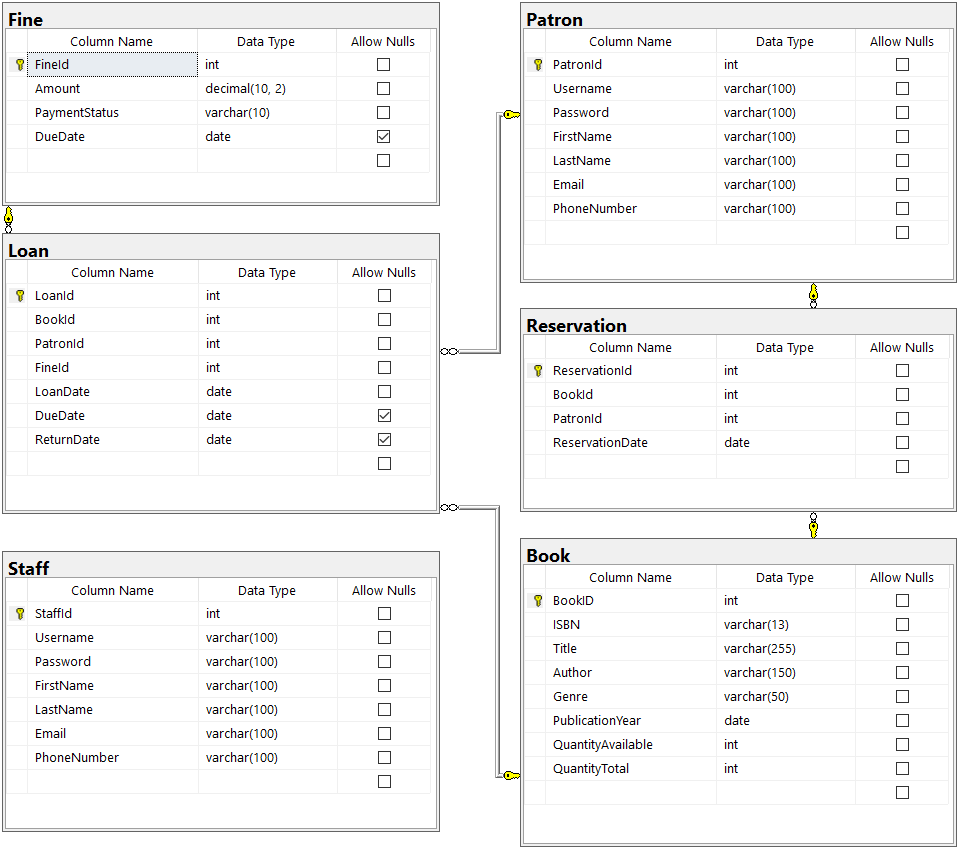
\includegraphics[width=.9\textwidth]{images/figures/Database Diagram.png}
\end{center}

\subsection{Database Implementation:}

\subsubsection{Table Creation Queries:}
\noindent
SQL queries were developed to create tables in the database, reflecting the structure outlined in the ERD. As an example, the query to create the Books table is provided below:

\begin{minted}[autogobble,breaklines]{SQL}
    CREATE TABLE
        [dbo].[Book]
    (
        [BookID]            INT             NOT NULL IDENTITY(1,1) PRIMARY KEY,
        [ISBN]              VARCHAR(13)     NOT NULL,
        [Title]             VARCHAR(255)    NOT NULL,
        [Author]            VARCHAR(150)    NOT NULL,
        [Genre]             VARCHAR(50)     NOT NULL,
        [PublicationYear]   DATE            NOT NULL,
        [QuantityAvailable] INT             NOT NULL,
        [QuantityTotal]     INT             NOT NULL
    );
\end{minted}
\noindent
Similar queries were created for other tables such as Patrons, Loans, and Fines, incorporating the necessary attributes and constraints.

\subsubsection{Data Seeding:}
\noindent
Initial data was seeded into the database to facilitate testing and demonstrate system functionality. Using SQL INSERT statements, sample data was added to tables. An example of seeding data into the Books table is illustrated below:

\begin{minted}[autogobble,breaklines]{sql}
    INSERT INTO [Book] (ISBN, Title, Author, Genre, PublicationYear, QuantityAvailable, QuantityTotal)
    VALUES  ('9781234567890', 'The Quantum Enigma', 'Olivia Sterling', 'Science Fiction', '2019', '48', '48'),
            ('9782345678901', 'Echoes of Eternity', 'Xavier Eclipse', 'Fantasy', '2017', '36', '36'),
            ('9783456789012', 'Cipher of Shadows', 'Seraphina Nightshade', 'Mystery', '2018', '36', '36');
\end{minted}
\noindent
Analogous seeding processes were followed for other relevant tables.

\newpage

\section{Web Development:}

\subsection{Front-End Technologies:}
\noindent
The front end of the web application was developed using a combination of HTML, CSS, and JavaScript. Bootstrap, a popular front-end framework, was also employed to enhance the visual appeal and responsiveness of the user interface.

\subsection{Back-End Technologies:}
\noindent
The back end of the application was implemented using a modified PHP:apache Docker image, following the MVC (Model-View-Controller) design pattern. This setup allowed for a seamless integration of the PHP scripting language with the Apache web server, providing a robust environment for server-side logic.

\subsection{User Authentication:}
\noindent
User authentication was an integral part of the system. The implementation involved configuring user roles and permissions within the PHP:apache Docker container, allowing for secure access control. Librarians and patrons were distinguished based on their assigned roles.

\subsection{Responsive Design:}
\noindent
The user interface was designed to be responsive, ensuring optimal display and functionality across a variety of devices and screen sizes. This was achieved through a combination of CSS media queries and Bootstrap's responsive design utilities.

\subsection{Docker Containerization:}
\noindent
The entire application was containerized using Docker, leveraging a multi-container architecture. Specifically, two Docker images were utilized: one for the modified PHP:apache environment hosting both frontend and backend components, and another running a SQL Server image to manage the database. This containerization facilitated efficient deployment, scalability, and consistent runtime environments across different systems.

\subsection{Integration:}
\noindent
The frontend, backend, and database components seamlessly interacted within the Dockerized environment. Docker Compose was employed to manage the multi-container application, ensuring the synchronization and communication between the PHP:apache and SQL Server containers.

\subsection{GitHub Version Control:}
\noindent
The assignment was collaboratively developed using GitHub for version control. A dedicated GitHub repository was established to track changes, manage branches, and facilitate seamless collaboration among team members.

\subsection{MVC Design Pattern:}
\noindent
The back-end architecture adhered to the MVC (Model-View-Controller) design pattern. This organizational structure facilitated the separation of concerns, promoting modular development, and ensuring a scalable and maintainable codebase.

\chapter{Design:}

\section{System Architecture:}
The system architecture was meticulously designed to ensure scalability, maintainability, and efficient communication between frontend and backend components. The architecture adopted a multi-container approach using Docker. The modified PHP:apache Docker image hosted both frontend and backend functionalities, while a separate Docker container ran a SQL Server image to manage the database. This modular design facilitated ease of deployment and maintenance.

The application adhered to the MVC (Model-View-Controller) design pattern, enhancing code organization and separation of concerns. The MVC architecture streamlined development, making the codebase more modular and extensible.

\newpage

\section{Database Schema:}

The database schema was derived from the earlier-created Entity-Relationship Diagram (ERD). SQL queries were crafted to implement the database schema within the SQL Server container. The schema was designed to accommodate tables for books, patrons, loans, fines, and other relevant entities, adhering to normalization principles for data consistency.

An illustrative snippet of the SQL query for creating the Books table, as part of the overall schema, is provided below:
\begin{minted}[autogobble,breaklines]{SQL}
    CREATE TABLE
        [dbo].[Book]
    (
        [BookID]            INT             NOT NULL IDENTITY(1,1) PRIMARY KEY,
        [ISBN]              VARCHAR(13)     NOT NULL,
        [Title]             VARCHAR(255)    NOT NULL,
        [Author]            VARCHAR(150)    NOT NULL,
        [Genre]             VARCHAR(50)     NOT NULL,
        [PublicationYear]   DATE            NOT NULL,
        [QuantityAvailable] INT             NOT NULL,
        [QuantityTotal]     INT             NOT NULL
    );
\end{minted}

\chapter{Implementation:}

\section{Coding Process:}
The coding process for the Library Management Software System involved the collaborative efforts of the development team. Following the design phase, the implementation kicked off with the creation of the backend logic using the PHP:apache Docker container. The MVC design pattern guided the organization of the codebase, separating concerns into models, views, and controllers.

Frontend development utilized HTML, CSS, JavaScript, and Bootstrap to craft a responsive and visually appealing user interface. The integration of frontend and backend components within the Dockerized environment ensured a cohesive and functional web application.

\section{Code Snippets:}
Below are snippets representing key aspects of the implementation. Please note that these are simplified examples for illustration:

\begin{minted}[autogobble,breaklines]{php}
    <?php

    class Database {
        private $host = DB_HOST;
        private $user = DB_USER;
        private $pass = DB_PASS;
        private $db_name = DB_NAME;

        private $dbh;
        private $stmt;

        public function __construct() {
            $dsn = 'sqlsrv:Server=' . $this->host . ';Database=' . $this->db_name . ';Encrypt=false';

            $option = [
                PDO::ATTR_ERRMODE => PDO::ERRMODE_EXCEPTION,
                PDO::ATTR_DEFAULT_FETCH_MODE => PDO::FETCH_ASSOC
            ];

            try {
                $this->dbh = new PDO($dsn, $this->user, $this->pass, $option);
            } catch (PDOException $e) {
                die($e->getMessage());
            }
        }

        public function query($query) {
        }

        public function bind($param, $value, $type = null) {
        }

        public function execute() {
        }

        public function resultSet() {
        }

        public function single() {
        }

        public function rowCount() {
        }

        public function lastInsertId() {
        }
    }
\end{minted}
These snippets provide a glimpse into the coding process, demonstrating how backend logic is structured using PHP and how frontend components interact with the backend through asynchronous JavaScript calls.

\chapter{Conclusion:}
The completion of the Library Management Software System assignment marks a significant milestone in our journey to leverage advanced database concepts and web development technologies. This section provides a summary of the assignment, highlighting key achievements and lessons learned throughout the development process.

\section{Summary of the assignment:}
The Library Management Software System was conceptualized and executed to fulfill the requirements of an advanced database course assignment. The assignment aimed to create a robust system that allows librarians to efficiently manage books, patrons, loans, and fines through a user-friendly web application. Leveraging Microsoft SQL Server for the database and incorporating a PHP:apache Docker image for the backend, the system seamlessly integrated diverse technologies to achieve a cohesive and functional solution.

The website, built with an MVC design pattern, offers a responsive and intuitive interface, ensuring a positive user experience. Librarians can perform essential CRUD operations on the database, and patrons benefit from features such as book reservations and due date notifications. The multi-container architecture, facilitated by Docker, provides scalability and streamlined deployment.

\section{Achievements:}

\subsection{Successful Implementation of CRUD Operations:}
\noindent
The system effectively implements Create, Read, Update, and Delete (CRUD) operations on the database, empowering librarians to manage library resources with ease.

\subsection{Responsive and Intuitive User Interface:}
\noindent
The website's frontend, developed using HTML, CSS, JavaScript, and Bootstrap, follows best practices for responsive design, ensuring a seamless experience across various devices.

\subsection{Secure User Authentication:}
\noindent
User authentication mechanisms were implemented, distinguishing between librarians and patrons. This ensures secure access control and protects sensitive operations.

\subsection{Containerized Deployment with Docker:}
\noindent
Leveraging Docker for containerization, the assignment achieved a modular and scalable deployment, enabling consistent runtime environments across different systems.

\section{Lessons Learned:}

\subsection{Challenges in Multi-Container Architecture:}
\noindent
Overcoming challenges in communication between Docker containers provided insights into optimizing multi-container architectures. This experience contributes to future assignments requiring containerized deployments.

\subsection{Integration of MVC Design Pattern:}
\noindent
Adhering to the MVC design pattern improved code organization and maintainability. This architectural choice proved beneficial in managing the complexity of the backend logic.

\subsection{Continuous Learning in Database Design:}
\noindent
Designing and implementing the database schema reinforced the importance of normalization for data consistency. Considerations for efficient data storage and retrieval were essential in creating a robust database.

\chapter{References and Appendicies}

\section{References:}
The successful completion of the Library Management Software System assignment was made possible through the utilization of various sources, frameworks, and libraries. The following references played a crucial role in the development process:


\subsection{W3Schools} 
\noindent \url{https://www.w3schools.com/}

A valuable online resource providing comprehensive tutorials and references for web development technologies, including HTML, CSS, and JavaScript. W3Schools served as a guide for implementing frontend components and ensuring adherence to industry best practices.


\subsection{MDN Web Docs by Mozilla}
\noindent \url{https://developer.mozilla.org/en-US/}

The MDN Web Docs offered authoritative documentation and guides for web technologies. It was an essential reference for understanding JavaScript functionalities, browser compatibility, and staying informed about the latest web standards.

\subsection{Bootstrap Documentation}
\noindent \url{https://getbootstrap.com/docs/5.3/getting-started/introduction/}

Bootstrap, a popular front-end framework, played a key role in designing a responsive and visually appealing user interface. The Bootstrap documentation provided guidance on implementing responsive design elements and components.

\subsection{Microsoft SQL Server Documentation}
\noindent \url{https://learn.microsoft.com/en-us/sql/sql-server/?view=sql-server-ver16}

The Microsoft SQL Server documentation was an invaluable resource for understanding and implementing database-related functionalities. It guided the creation of the database schema, SQL queries, and interactions with the SQL Server container.
These references collectively contributed to the successful development and implementation of the Library Management Software System. Each source played a significant role in guiding decision-making processes, ensuring best practices, and fostering a deeper understanding of the technologies employed.

\section{Appendices:}
For additional materials please refer to the GitHub repository associated with the assignment. The appendices in the repository provide a comprehensive resource for further exploration and understanding of the assignment's intricacies.
\noindent \url{https://github.com/G4CENeiz/advanced-database-web-app}

\end{document}